\chapter{Synthèse et optimisation des circuits séquentiels}
\section{Classes et représentation}
Rappelons que l'état du système n'est pas forcement visible par l'extérieur.\\
La sortie d'un système est fonction de l'état et \textit{éventuellement} des entrées. Cet \textit{éventuellement} implique 2 classes de circuit logique séquentiel:
\begin{itemize}
	\item Machine de Moore (pas Gordon!)
	\item Machine de Meally
\end{itemize}
\paragraph{Machine de Moore:}
la \textbf{sortie} est \textbf{uniquement} fonction des \textbf{variables d'état}.
\begin{figure}[H]
	\centering
	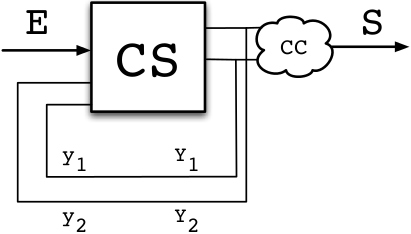
\includegraphics[width=.3\textwidth]{ch7/image1}
\end{figure}
\paragraph{Machine de Meally:}
la \textbf{sortie} est fonction (combinatoire) des \textbf{variables d'état} et des \textbf{entrées}.
\begin{figure}[H]
	\centering
	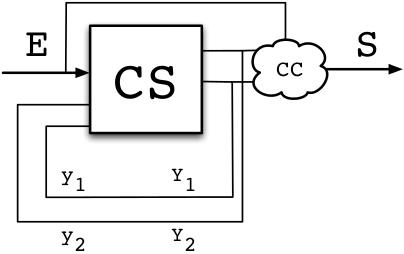
\includegraphics[width=.3\textwidth]{ch7/image2}
\end{figure}

Pour la synthèse à partir d'un cahier de charges verbal :
\begin{enumerate}
	\item Table d'état (ou Table de Huffman)
	\item Graphe d'état (optionnel)
	\item Équations logiques (et le circuit logique)
\end{enumerate}
\subsection{Codage des états}
On souhaite représenter les systèmes séquentiels à l'aide des codes binaires $\{0, 1, \text{-}\}$. Ce processus d'attribution de codes binaires aux états codés s'appelle \textit{le codage des états}.\\
Le nombre de bits nécessaires pour coder $n$ états est donné par $\log_2n$.
\subsubsection{Exemple}
Soit un système à 4 états. Attribuons à chaque état un code binaire (4 états $\rightarrow \log_2 4=2\rightarrow$ 2 bits nécessaires).\\
Ainsi $1\rightarrow 00,\ 2\rightarrow 01,\ 3\rightarrow 11,\ 4\rightarrow 10$.\\
Ainsi, on obtient:
\begin{figure}[H]
	\centering
	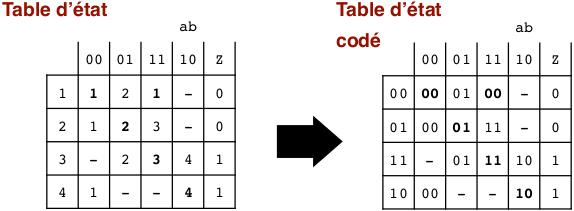
\includegraphics[width=.6\textwidth]{ch7/image3}
\end{figure}
À chaque bit du code correspond une fonction logique. On a donc : 4 états et 2 variables d'états ($y_2y_1$)$\rightarrow$ 2 fonctions logiques.
\begin{figure}[H]
	\centering
	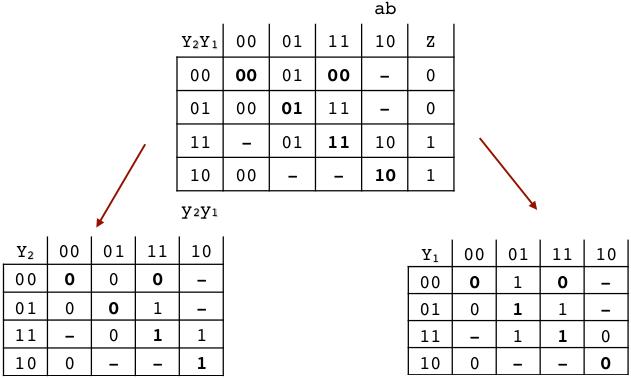
\includegraphics[width=.7\textwidth]{ch7/image4}
\end{figure}
Il suffit de simplifier la K-Map de $Y_2$ et celle de $Y_1$ et déduire leur fonction logique respective
\begin{figure}[H]
	\centering
	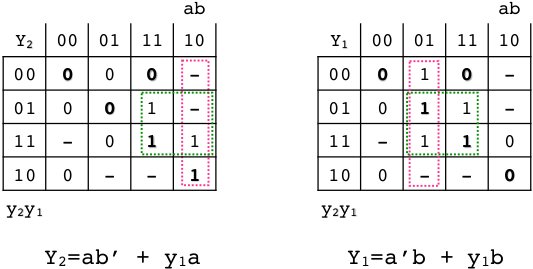
\includegraphics[width=.7\textwidth]{ch7/image5}
\end{figure}
\danger $y_2y_1\neq Y_2Y_1$, les premières représentent le présent, les 2 autres le futur.\\

Établissons la \textit{fonction de sortie}. Connaissant la valeur de sortie des états stables, nous pouvons remplir les cases correspondantes.
\begin{figure}[H]
	\centering
	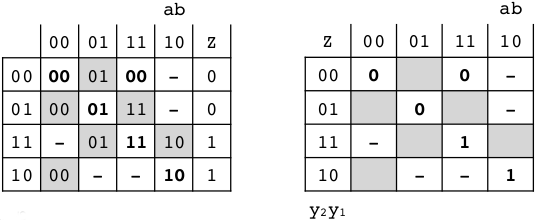
\includegraphics[width=.7\textwidth]{ch7/image6}
\end{figure} Pour les transitions (cases grises), il faut respecter les transitions ainsi que la règle suivante:
\begin{center}
	\textbf{Lors des transitions, si la sortie doit changer, elle ne devrait changer qu'une seule fois}
\end{center}
c-à-d que les \textbf{seules} possibilités sont
\begin{figure}[H]
	\centering
	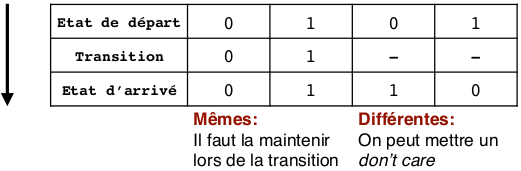
\includegraphics[width=.7\textwidth]{ch7/image7}
\end{figure}
Nous obtenons donc
\begin{figure}[H]
	\centering
	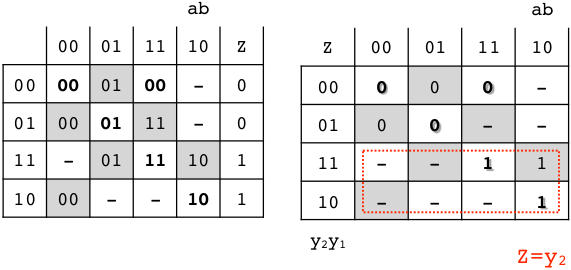
\includegraphics[width=.7\textwidth]{ch7/image8}
\end{figure}
Le logigramme correspondant n'est autre que
\begin{figure}[H]
	\centering
	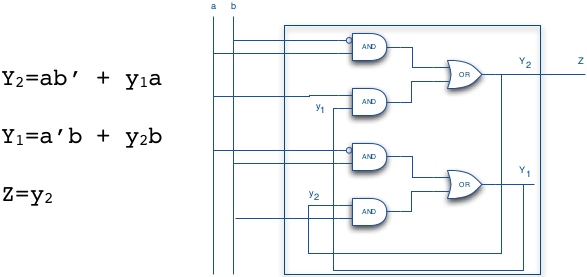
\includegraphics[width=.8\textwidth]{ch7/image9}
\end{figure}
\section{Simplification de la table primitive des états}
L’algorithme de synthèse se constitue de 3 étapes :
\begin{enumerate}
	\item Table primitive d'état ou Table de Huffman :
	\begin{itemize}
		\item Écrire la table de Huffman à partir d'un cahier de charges.
		\item La \textbf{1\up{ère}} table ne peut avoir qu'\textbf{un seul état stable par ligne de la table d'état}
	\end{itemize}
	\item Codage des états
	\item Équations logiques
\end{enumerate}
La complexité du circuit obtenu lors de la synthèse est influencé par la complexité (taille) de la taille initiale d'état.\\
Chaque bit de code ($\log_2n$ bits de code pour $n$ états) représente:
\begin{itemize}
	\item une fonction logique
	\item un organe de mémoire (délais)
\end{itemize}
Il faut donc réduire le nombre d'états pour simplifier le circuit correspondant.
\subsection{Réduction du nombre d'état}
\subsubsection{Notion d'équivalence de deux états}
Deux états sont équivalents si (équivalence de deux états stables):
\begin{enumerate}
	\item ils produisent la \textbf{même sortie}
	\item pour \textbf{toutes} combinaisons des variables d'entrée, les \textbf{futurs} états sont soit les mêmes soit \textbf{équivalents}
\end{enumerate}
Nous obtenons donc deux types d'équivalence:
\begin{itemize}
	\item \textbf{États identique} : 2 (ou plus) états stables sont au même endroit (même combinaison des entrées)
	\begin{figure}[H]
		\centering
		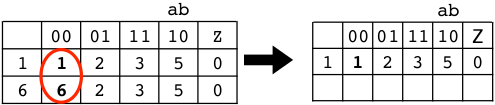
\includegraphics[width=.7\textwidth]{ch7/image10}
	\end{figure}
	\item \textbf{États fusionnables} : les états stables se trouvent à des endroits différents (combinaison des entrées différentes)
	\begin{figure}[H]
		\centering
		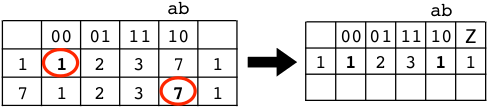
\includegraphics[width=.7\textwidth]{ch7/image11}
	\end{figure}
\end{itemize}
Pour que $n$-états soient équivalents il faut que tous les états soient équivalents deux à deux.\\

Pour ce faire, on dresse un tableau de $n(n-1)/2$ cases appelé \textbf{table des conditions d'équivalences}:
\begin{itemize}
	\item Chaque case de la table représente la possibilité d'équivalence et/ou de fusionnement de deux états
	\item \textbf{Dans le cas de la machine de Moore}, toute paire d'états ayant la sortie différente peut être exclue
	\item L'impossibilité de fusionner deux états se note par une croix
\end{itemize}
Pour 11 états, la table des conditions d'équivalence ressemble à:
\begin{figure}[H]
	\centering
	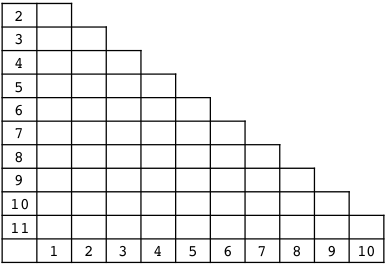
\includegraphics[width=.6\textwidth]{ch7/image12}
\end{figure}
\section{Synthèse d'un flip-flop D}
\begin{wrapfigure}{r}{.5\textwidth}
	\centering
	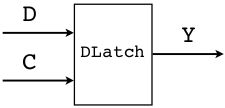
\includegraphics[width=.3\textwidth]{ch7/image13}
\end{wrapfigure}
\subsection{D-Latch:} Mémoire suiveuse-bloqueuse (\textit{Sample and Hold}).\\
Spécification:
\begin{itemize}
	\item 2 entrées : D (\textit{data}) et C (\textit{control})
	\item Une sortie : Y
	\item La sortie prend la valeur de l'entrée D lorsque C$=1$
\end{itemize}
\subsection{D Flip-Flop (\textit{edge triggered})}
\begin{wrapfigure}{r}{.5\textwidth}
	\centering
	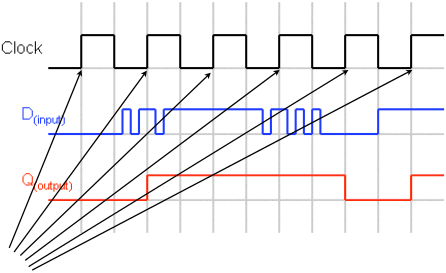
\includegraphics[width=.4\textwidth]{ch7/image14}
\end{wrapfigure}
Spécification :
\begin{itemize}
	\item La sortie prend la valeur de D \textbf{uniquement} lors d'un \textbf{flanc montant} de C (passage de $0\rightarrow 1$)
	\item Entre 2 flancs montants, la valeur de D est maintenue (toute variation de D est ignorée)
	\item Si C est sur un flanc montant et que D varie, la sortie prend l'ancienne valeur de D, celle juste avant le flanc montant 
	\item Le reste n'est que maintient
\end{itemize}
\subsubsection{Table primitive d'état}
\begin{minipage}{.5\textwidth}
	Considérons l'évolution qui mettra la sortie à 1:
\begin{enumerate}
	\item Situation de départ $\rightarrow Q=0$ et aucun changement à l'entrée (le $CD=00$ ne change pas) $\Rightarrow$ état 1
	\item $D$ change ($0\rightarrow 1$) avant $C$ $\Rightarrow$ état 2
	\item $C$ change $\Rightarrow$ état 4
\end{enumerate}
\end{minipage}
\vspace{-2.9cm}
\begin{minipage}{.5\textwidth}
	\begin{figure}[H]
		\centering
		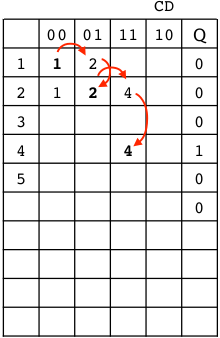
\includegraphics[width=.7\textwidth]{ch7/image15}
	\end{figure}
\end{minipage}
\begin{minipage}{.5\textwidth}
	Considérons maintenant une autre évolution en partant de l'état 1
	\begin{enumerate}
		\item $C$ change avant $D$ ($CD=00\rightarrow 10$) $\Rightarrow$ état 3
		\item $D$ change, le système ignore sa variation $\Rightarrow$ état 5 (diffère de l'état 4 par la valeur de la sortie $Q$)
	\end{enumerate}
\end{minipage}
\begin{minipage}{.5\textwidth}
	\begin{figure}[H]
		\centering
		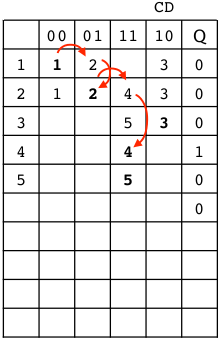
\includegraphics[width=.7\textwidth]{ch7/image16}
	\end{figure}
\end{minipage}

\begin{minipage}{.5\textwidth}
	Principe de mémorisation d'un 1
	\begin{enumerate}
		\item Initialement : $CD=00$
		\item $CD=00\rightarrow 01\rightarrow 11$
		\item $Q=0\rightarrow 1$ (état 4)
		\item $C=0 \Rightarrow$ peu importe la valeur de $D$, la sortie reste à 1 (états 7 et 9)
	\end{enumerate}
\end{minipage}
\begin{minipage}{.5\textwidth}
	\begin{figure}[H]
		\centering
		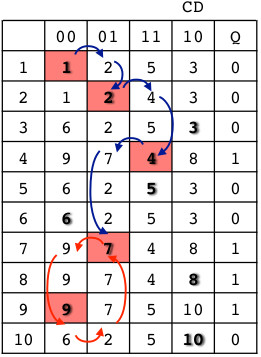
\includegraphics[width=.7\textwidth]{ch7/image17}
	\end{figure}
\end{minipage}

\subsubsection{Table de conditions d'équivalences}
Cette table se définit en 3 passes:
\begin{enumerate}
	\item[-- Passe 1.] Sorties différentes
	\begin{figure}[H]
		\centering
		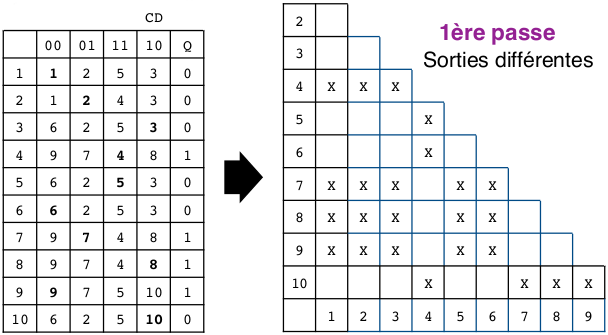
\includegraphics[width=.7\textwidth]{ch7/image18}
	\end{figure}
	\item[-- Passe 2.] Conditions de fusionnements 
	\begin{figure}[H]
		\centering
		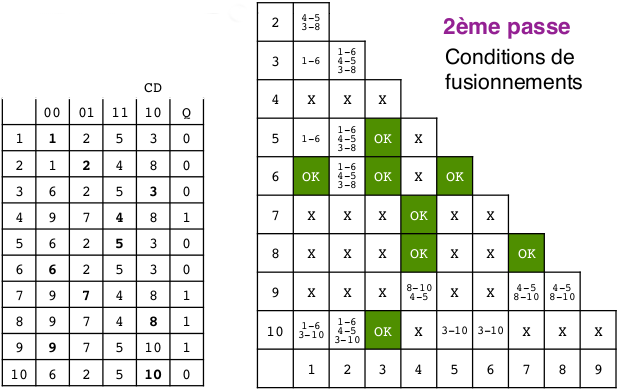
\includegraphics[width=.7\textwidth]{ch7/image19}
	\end{figure}
	\item[-- Passe 3.] Suppression des impossibles
	\begin{figure}[H]
		\centering
		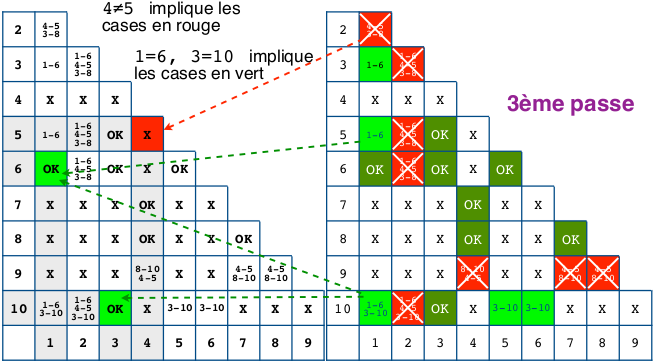
\includegraphics[width=.7\textwidth]{ch7/image20}
	\end{figure}
\end{enumerate}
Nous pouvons donc obtenir de ce tableau une liste assez claire des fusionnements possibles :
\begin{figure}[H]
	\centering
	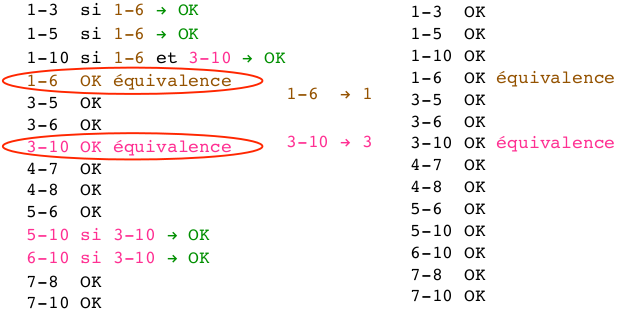
\includegraphics[width=.7\textwidth]{ch7/image21}
\end{figure}
Après avoir établi nos choix de fusionnement, il suffit de les appliquer à la table primitive d'état et de réordonner pour plus de lisibilité :
\begin{figure}[H]
	\centering
	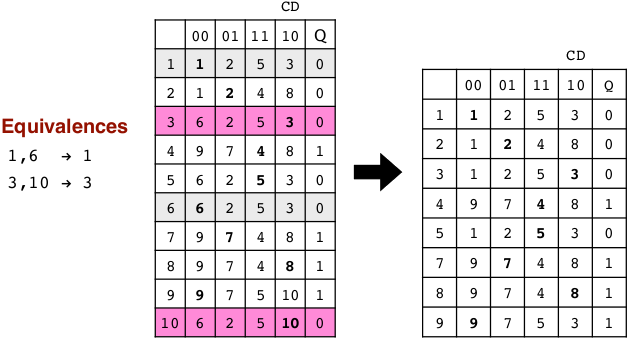
\includegraphics[width=.7\textwidth]{ch7/image22}
\end{figure}
Nous passons donc de 10 à 4 états $\Rightarrow$ 2 variables d'état au lieu de 4 !\\

Le choix du codage des états étant (pour l'instant) arbitraire : $1\rightarrow 00,\ 2\rightarrow 01,\ 3\rightarrow 11,\ 4\rightarrow 10$. Il ne reste plus qu'à écrire la K-Map de chaque variable d'état et d'en déduire leur fonction logique:
 \begin{figure}[H]
 	\centering
 	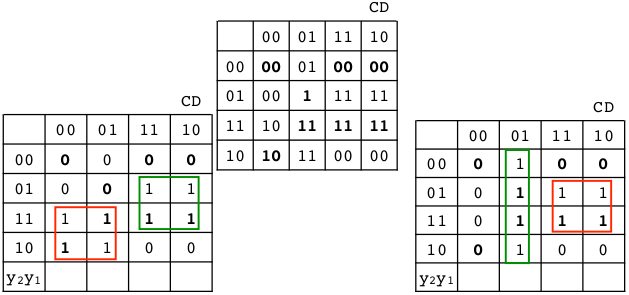
\includegraphics[width=.7\textwidth]{ch7/image23}
 \end{figure}
\section{Différents organes de mémoire}
Nous verrons 4 type de flip-flop :
\begin{itemize}
	\item SR : $Q=1$ lorsque $S=1$. La combinaison $SR=11$ est interdite.
	\item JK : même chose que SR mais la combinaison interdite change d'état
	\item D : la sortie suit l'entrée
	\item T : changement d'état lorsque l'entrée $T=1$
\end{itemize}
\subsection{Description des flip-flops}
Nous verrons 3 manières pour décrire un flip-flop :
\begin{itemize}
	\item Table de fonctionnement (sorte de table d'état)
	\item Équations caractéristiques
	\item Table d'excitation 
\end{itemize}
On notera l'état présent par un Q et l'état futur par un Q\up{+}. À cela s'ajoute (pour la table d'excitation) 4 possibilités de couple présent-futur
\begin{figure}[H]
	\centering
	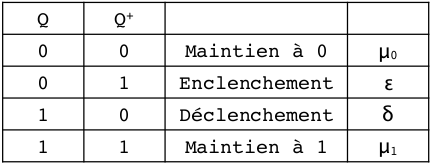
\includegraphics[width=.5\textwidth]{ch7/image24}
\end{figure}
\subsubsection{Flip-flop SR}
\begin{figure}[H]
	\centering
	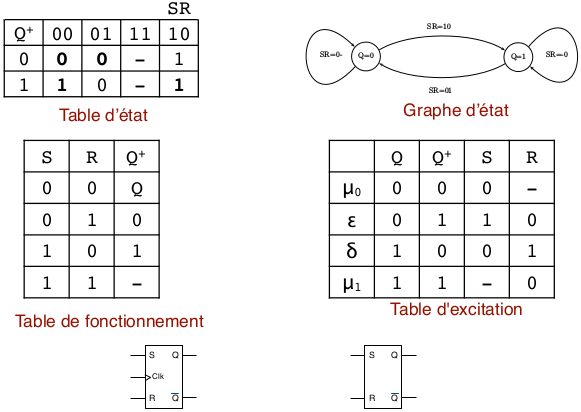
\includegraphics[width=.8\textwidth]{ch7/image25}
	\caption{Représentation schématique flip-flop SR}
\end{figure}
\subsubsection{Flip-flop JK}
\begin{figure}[H]
	\centering
	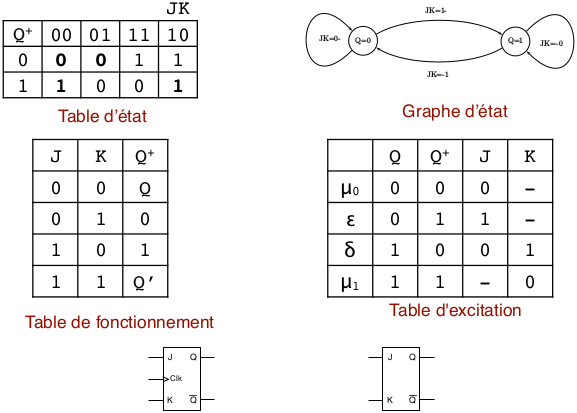
\includegraphics[width=.8\textwidth]{ch7/image26}
	\caption{Représentation schématique flip-flop JK}
\end{figure}
\subsubsection{Flip-flop D}
\begin{figure}[H]
	\centering
	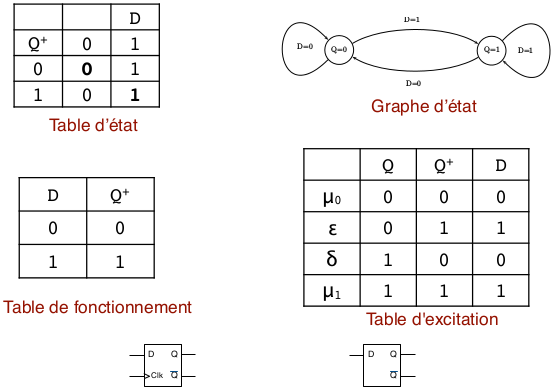
\includegraphics[width=.8\textwidth]{ch7/image27}
	\caption{Représentation schématique flip-flop D}
\end{figure}
\subsubsection{Flip-flop T}
\begin{figure}[H]
	\centering
	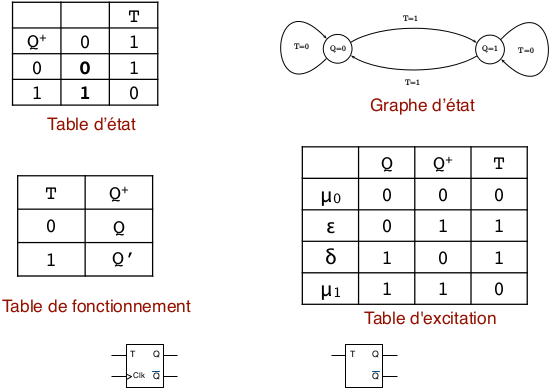
\includegraphics[width=.8\textwidth]{ch7/image28}
	\caption{Représentation schématique flip-flop T}
\end{figure}
\section{Courses critiques}
L'un des problèmes fondamental des circuits réels logiques à rétroaction est le problème des courses critiques. Il existe 2 méthodes de résolution des courses critiques 
\begin{itemize}
	\item Action sur le \textbf{codage des états} et les transitions $\Rightarrow$ conception des systèmes \textbf{séquentiels asynchrones}
	\item Action sur la \textbf{mise à jour} des variables d'état $\Rightarrow$ conception des systèmes \textbf{séquentiels synchrones}
\end{itemize}
\subsection{Origine du problème des courses critiques}
